\chapter{Electrical Design}
This section describes the electrical design, layout and components used for the fixed and variable pitch quadcopters. Additionally, a mass budget have been calculated for the two quadcopters.

\section{Fixed Pitch Quadcopter}
In Fig. \ref{fig:fpqsch} the schematic for the quadcopter concept described in section \ref{sec;FPQply} is displayed.

\begin{figure}[H]
    \centering
    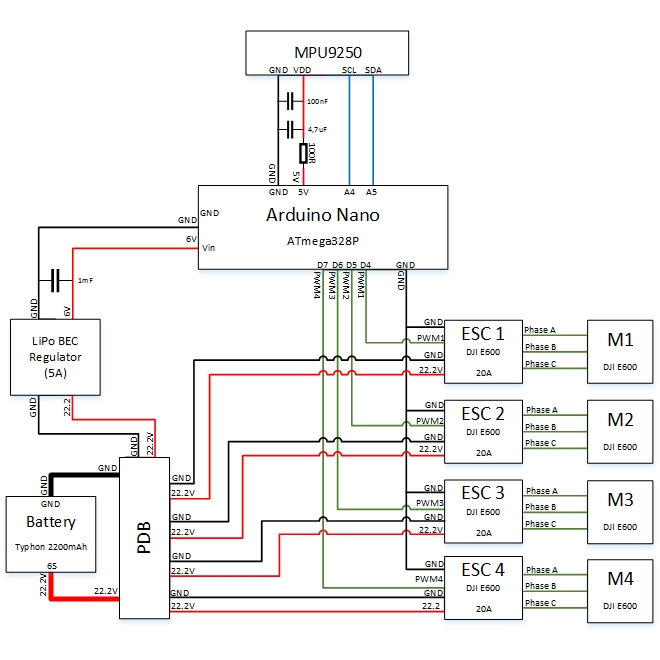
\includegraphics[width = 0.8\textwidth]{VAPIQ-PICTURES/shemfpq}
    \caption{Schematic for first FPQ}
    \label{fig:fpqsch}
\end{figure}

In Tab. \ref{tab:CompFPQ} the electrical components needed to construct the FPQ are displayed. The components were chosen based on the DJI E600 motors. The electronics were placed on a breadboard for easy design change.
\begin{table}[H]
    \begin{center}
    \caption{Components used for FPQ} 
    \label{tab:CompFPQ} 
        \begin{tabular}{|l|l|c|}
            \hline 
            \cellcolor{white}\textbf{Component:} & \textbf{Info:} & \textbf{Qty.:}  \\ 
            \hline
            Motor & DJI E600  & 4 \\
            ESC & E600 20A & 4 \\
            Bluetooth Module & HC-06 & 1  \\
            Microcontroller & Arduino Nano  ATmega328P& 1 \\
            LiPo Battery & Gens ace 4600mAh, 6S, 35C & 1 \\
            LiPo BEC Regulator & In: 6v-25v, Out: 6V (Max. 5A)  & 1\\
            IMU & MPU9250 & 1 \\
            \hline
        \end{tabular}
    \end{center}
\end{table}

To be able to compute the required thrust at hover, the total mass had to be determined. In Tab. \ref{tab:WeightFPQ} the mass budget for the FPQ is displayed. 

\begin{table}[H]
    \begin{center}
    \caption{Mass budget FPQ} 
    \label{tab:WeightFPQ} 
        \begin{tabular}{|l|c|c|}
            \hline 
            \textbf{Component:} & \textbf{Qty.:} & \textbf{Mass[g]:}  \\ 
            \hline
            Frame + cables & 1 & 611.2\\
            Propellers & 4 & 82.8\\
            DJI E600  & 4 & 360 \\
            E600 20A ESC & 4 & 80 \\
            Bluetooth Module HC-06 & 1 & 2\\
            MPU 9250 & 1 & 2 \\
            Arduino Nano & 1 & 7 \\
            LiPo Battery & 1 & 670 \\
            LiPo BEC Regulator & 1 & 19 \\
            PDB & 1 & 20 \\\hline
            \textbf{Total mass budget:} & & 1856\\
            \hline
        \end{tabular}
    \end{center}
\end{table}

From the mass budget in Tab. \ref{tab:WeightFPQ} and the maximum power measured in \ref{app:tr005} for the DJI E600 motors, the power to weight ratio can be calculated.

\begin{equation}
    Ratio = \frac{Power}{Weight} = \frac{4\cdot1640g}{1856g}=3.5
\end{equation}

\newpage

\section{Variable Pitch Quadcopter}
In Fig. \ref{fig:vpqsch} the schematic for the quadcopter concept described in section \ref{sec;VPQply} is displayed. This diagram is designed based on the AXI 2208/26 motors. To be able to get the most accurate and comparable data, the same quadcopter is used as a fixed pitch quadcopter. This ensures a physically equal quadcopter. By choosing a fixed angle for the propellers and only changing the RPM, the quadcopter will work as a traditionally fixed pitch quadcopter. 
\begin{figure}[H]
    \centering
    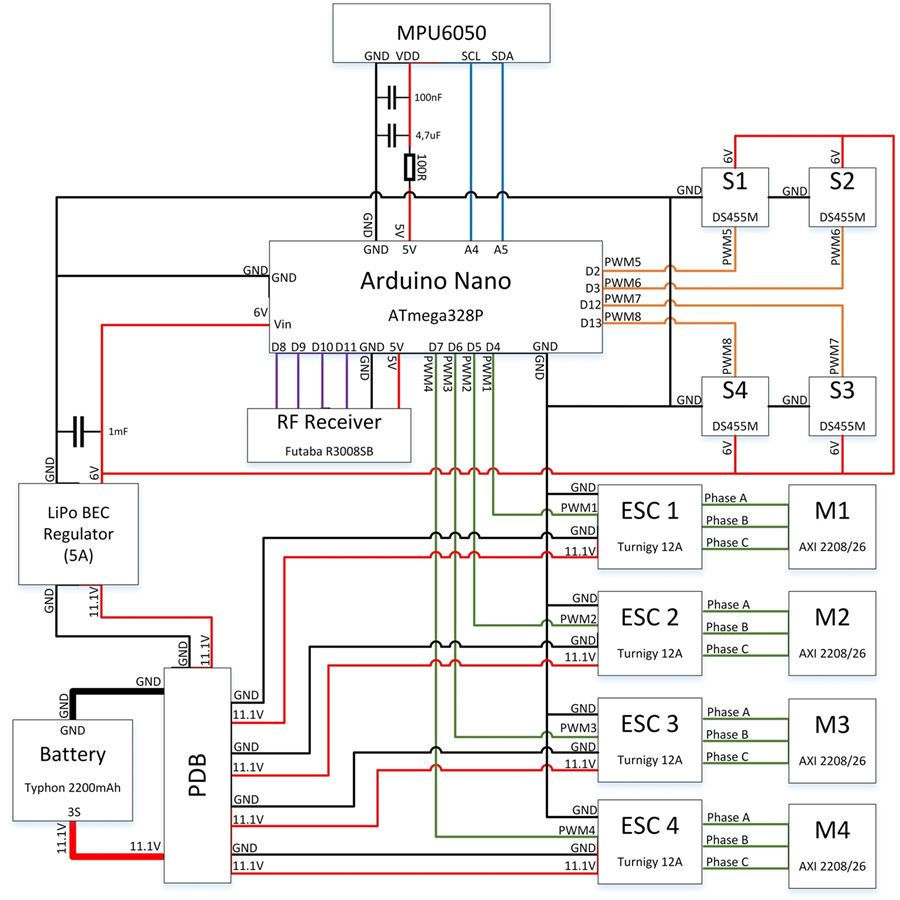
\includegraphics[width = 1\textwidth]{VAPIQ-PICTURES/Shematic}
    \caption{Schematic for VPQ}
    \label{fig:vpqsch}
\end{figure}

In Tab. \ref{tab:CompVPQ} the electrical components for the VPQ are displayed. The components in this table are chosen based on the AXI 2208/26 motors. 
\begin{table}[H]
    \begin{center}
    \caption{Components used for VPQ} 
    \label{tab:CompVPQ} 
        \begin{tabular}{|l|l|c|}
            \hline 
            \textbf{Component:} & \textbf{Info:} & \textbf{Qty.:}  \\ 
            \hline
            Motor & AXI 2208/26 Gold Line & 4 \\
            ESC & Turnigy Opto 12A & 4 \\
            Servo & Align DS455M, 2.9kg/0.04s & 4  \\ 
            Radio Receiver & Futaba R3008SB & 1  \\
            Microcontroller & Arduino Nano  ATmega328P& 1 \\
            LiPo Battery & Typhon 2200mAh, 3S, 25C & 1 \\
            LiPo BEC Regulator & In: 6v-25v, Out: 6V (Max. 5A)  & 1\\
            IMU & MPU6050 & 1 \\
            \hline
        \end{tabular}
    \end{center}
\end{table}


To identify the required thrust for hover, the total mass needs to be calculated. In Tab. \ref{tab:WeightVPQ} the mass budget for the VPQ is displayed.
\begin{table}[H]
    \begin{center}
    \caption{Mass budget VPQ} 
    \label{tab:WeightVPQ} 
        \begin{tabular}{|l|c|c|}
            \hline 
            \textbf{Component:} & \textbf{Qty.:} & \textbf{Mass[g]:}  \\ \hline
            Frame & 1 & 83\\
            Propellers + EVP mechanism & 4 & 60\\
            AXI 2208/26 Gold Line  & 4 & 180 \\
            Turnigy Multistar ESC & 4 & 20\\
            Servo & 4 & 80 \\
            RF Receiver Futaba R3008SB & 1 & 11\\
            MPU6050 & 1 & 2 \\
            Arduino Nano & 1 & 7 \\
            LiPo Battery & 1 & 153 \\
            LiPo BEC Regulator & 1 & 19 \\
            Miscellaneous & N/A & 148 \\\hline
            \textbf{Total mass budget:} & & 763 \\
            \hline
        \end{tabular}
    \end{center}
\end{table}

From Tab. \ref{tab:WeightVPQ} and the maximum power measured for the AXI 2208/26 motors, the power to weight ratio can be calculated.

\begin{equation}
    Ratio = \frac{Power}{Weight} = \frac{4\cdot550g}{763g}=2.88
\end{equation}

%As a thumb rule, the power to weight ratio should be more than 2 to be able to have stable flight. 
\newpage

\section{Electronic Component Description for VPQ}
Since the Variable Pitch Quadcopter is used to for both fixed and variable pitch, a further analysis is done for the components on this quadcopter.\bigskip

\textbf{Arduino Nano}\\
The microcontroller used for the flight controller is an Arduino Nano. It was chosen for its size and acceptable computational power \cite{Arduino}. The specifications for the microcontroller are listed in Tab. \ref{tab:nanospecs}.

\begin{table}[H]
    \begin{center}
    \caption{Arduino Nano Specs} 
    \label{tab:nanospecs} 
        \begin{tabular}{|l|l|}
            \hline 
                Microcontroller & ATmega328P\\
                Operating Voltage & 5V \\
                SRAM & 2 KB\\
                Clock Speed & 16MHz \\
                Analog I/O Pins & 8\\
                Digital I/O Pins & 22\\
                EEPROM & 1 KB\\
                Input Voltage & 7-12V\\
                Weight & 7g\\
                Size & 18x45 mm\\
            \hline
        \end{tabular}
    \end{center}
\end{table}\bigskip


\textbf{AXI 2208/26 Motors}\\
The motors chosen for the variable pitch quadcopter are brushless hobby motors from AXI with hollow shafts. The specific model is AXI 2208/26 Gold Line EVP. These motors have a Kv rating of 1420. Kv is the no-load RPM/V. These motors have a high power output, but are light weight. The total weight of one motor with cables is 45 grams. From these specification and a 3S LiPo battery the maximum no-load RPM can be calculated to be

\begin{equation}
   RPM_{no-load} = Kv \cdot Battery \: Voltage = 1420\: RPM/V \cdot 11.1V = 15 762 \:RPM = 1650.6 \: rad/s
\end{equation}\bigskip


\textbf{ESC}\\
The electronic speed controllers chosen for the AXI motors are from Turnigy Multistar, with input voltage of two to four cells LiPo battery, constant current of 12A and a weight of 6 grams. They support a 480Hz refresh rate with a resolution of 32 bit. \bigskip


\textbf{Servos}\\
To actuate the pitch mechanism, four Align DS455M Digital Servos are used. These are metal geared digital servos and the spesifications are displayed in Tab. \ref{tab:servospecc}. 

\begin{table}[H]
    \begin{center}
    \caption{Align DS455M Digital Servo spec} 
    \label{tab:servospecc} 
        \begin{tabular}{|l|l|}
            \hline 
               Weight & 20g \\
               Dimension & 23 x 12 x 31.3mm \\
                Operating voltage & DC 6.0V \sim 8.4V \\
                Torque & 2.2Kg.cm @ 6.0V; 2.9Kg.cm @ 8.4V \\
                Motion speed & 0.05sec/60^\circ @6.0V; 0.04sec/60^\circ @ 8.4V \\
                Temperature Range & -20^\circ C \sim +60^\circ C \\
            \hline
        \end{tabular}
    \end{center}
\end{table}\bigskip

\textbf{IMU}\\
The Inertial Measurement Unit chosen for the variable pitch quadcopter is a MPU6050. The MPU6050 has six degrees of freedom. This sensor has a 3-axis gyroscope and a 3-axis accelerometer. By having an accelerometer and a gyroscope in the same sensor, it eliminates the problem of cross-axis errors when using separate devices, because both are based around the same axes. The gyroscope has an update frequency of 8kHz and the accelerometer has an update frequency of 1kHz. When the loop is running at 250 Hz, the number of samples for processing is 32 and 4 respectively.\bigskip

\textbf{LiPo BEC Regulator}\\
The servos need 6V to be actuated. To distribute the right voltage to the servos, a LiPo BEC Regulator is used. The LiPo BEC Regulator can handle voltage inputs between 6-25V and it can distribute a constant voltage output of 6V. The maximum output current is 5A. The Regulator is also used to power the Arduino Nano. The Arduino Nano has a maximum current draw of 400mA and the servos have a maximum current draw of 1A when a large load is applied. Eq. \ref{eq:ITOT} shows that 5A from the BEC Regulator is enough to power both the servos and the Arduino Nano. 

\begin{equation}
\label{eq:ITOT}
   I_{tot} = I_{servo}\cdot4 + I_{Arduino} = 1A\cdot4 + 0.40A = 4.4A 
\end{equation}\bigskip


\textbf{LiPo Battery}\\
Based on the electronic components described above and the need for a light weight LiPo battery, the Typhon 2200 mAh was chosen. The specifications for the battery is provided in Tab. \ref{tab:lipospecs}. 
\begin{table}[H]
    \begin{center}
    \caption{LiPo Battery Specs} 
    \label{tab:lipospecs} 
        \begin{tabular}{|l|l|}
            \hline 
                Capacity & 2200 mAh \\
                Voltage & 11.1V \\
                Number of cells & 3 \\
                C-Rating & 25 \\
                Weight & 153 grams \\
            \hline
        \end{tabular}
    \end{center}
\end{table} \bigskip

A set of calculations have also been executed to ensure that the chosen battery can deliver enough power to the whole system. \bigskip

The constant discharge rate when using a 2200 mAh 25C LiPo battery can be calculated to be

\begin{equation}
    \frac{2200\:mAh \cdot 25 C}{1000} = 55 A
\end{equation} \bigskip

The total current draw for the quadcopter is dependant on the way it is being flown and other effects like drag, weight and wind. The approximately maximum flying time of one battery can anyhow be calculated based on the current draw from all the components. Each motor have a maximum current draw of 12A, so the total maximum current draw for all four AXI motors are
\begin{equation}
    I_{M}_{max} = 4 \cdot 12A = 48 A
\end{equation}

Maximum current draw for all components are
\begin{equation}
  I_{tot} = I_{M}_{max} + I_{BEC} =  48A + 5A = 53A  
\end{equation}

This means that the approximately maximum flying time can be calculated to be
\begin{equation}
  t_{max} = \frac{2.2Ah}{53A}\cdot60 = 2.5\:minutes
\end{equation}

Assuming that only 60 percent of the maximum current draw for all components are used, since the throttle values are limited to about 60 percent, the flight time will be
\begin{equation}
  t_{60} = \frac{2.2Ah}{31.8A}\cdot60 = 4.15 \: minutes
\end{equation}

\newpage
